\documentclass[tikz,border=10pt]{standalone}
\usepackage{tikz}
\usepackage{amsmath}
\usetikzlibrary{shapes.geometric,arrows.meta,positioning,fit,backgrounds,shadows,decorations.pathreplacing,calc}

\begin{document}
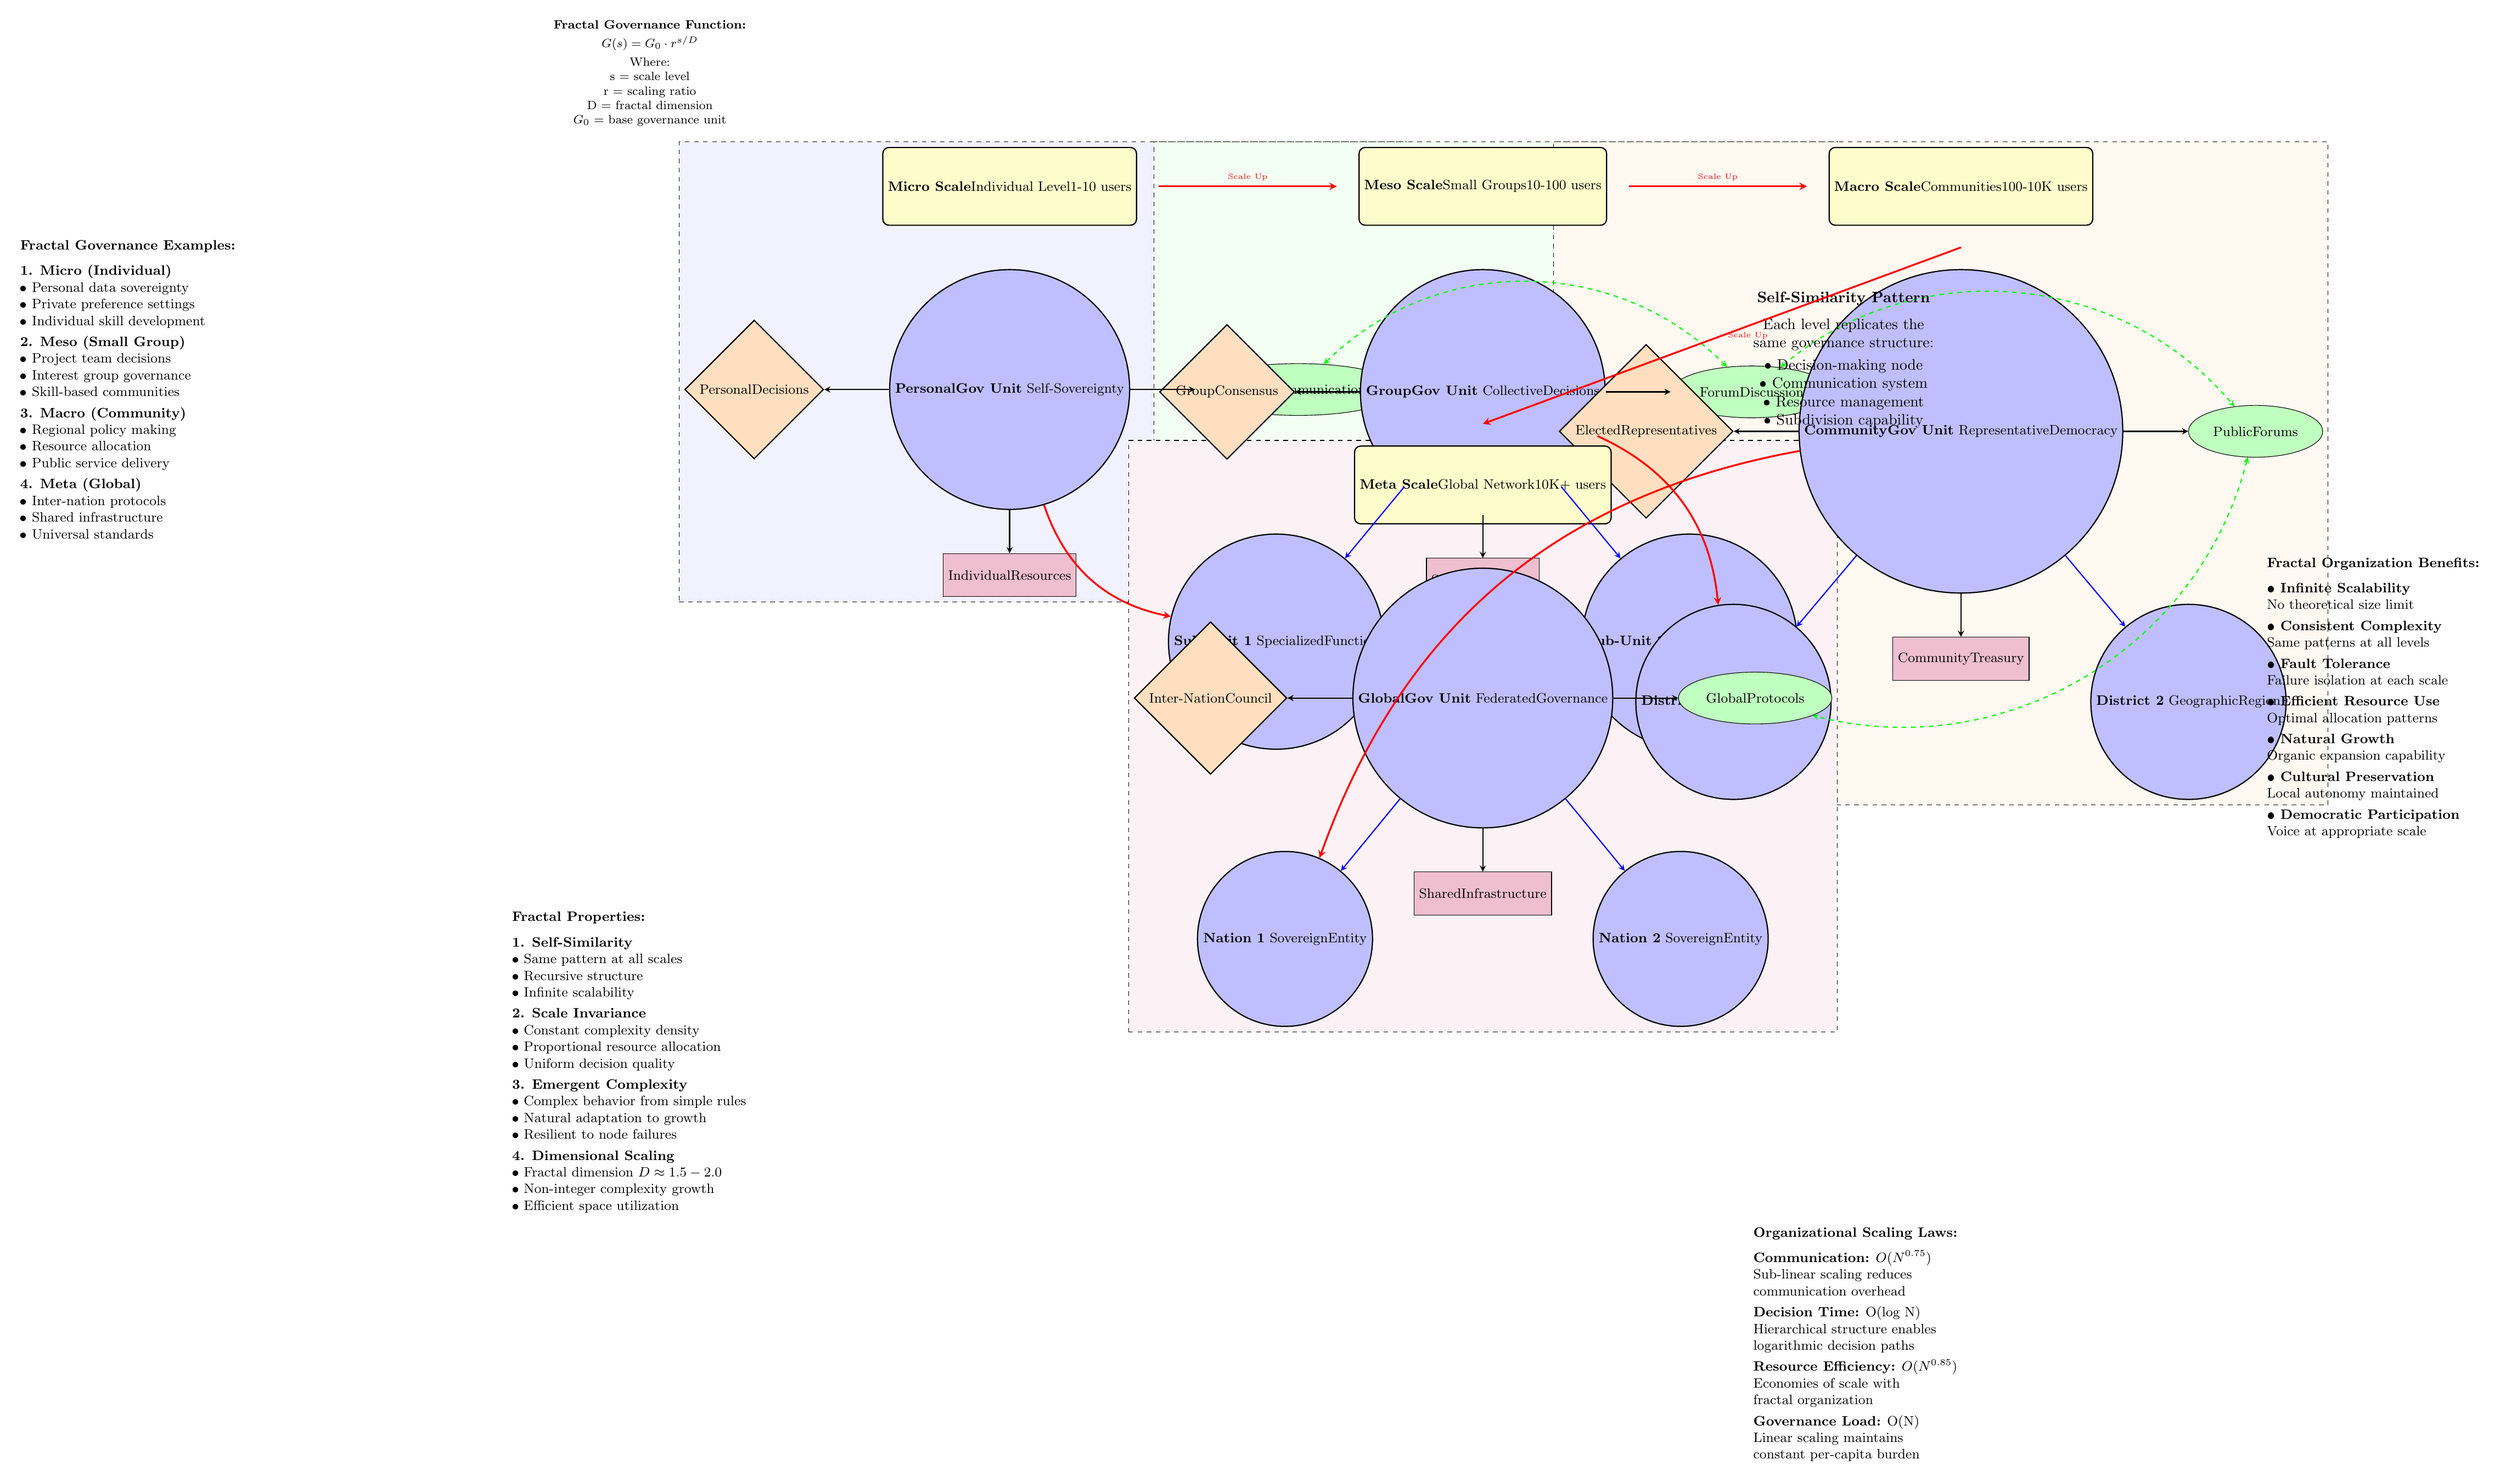
\begin{tikzpicture}[scale=1,
    node distance=5cm,
    every node/.style={font=\small},
    % Fractal organization components
    governance_unit/.style={circle,draw,minimum size=2.5cm,fill=blue!25,thick},
    decision_node/.style={diamond,draw,minimum size=1.8cm,fill=orange!25,thick},
    communication/.style={ellipse,draw,minimum width=2cm,minimum height=1.2cm,fill=green!25},
    resource/.style={rectangle,draw,minimum width=1.8cm,minimum height=1cm,fill=purple!25},
    scale_indicator/.style={rectangle,draw,minimum width=3.5cm,minimum height=1.8cm,fill=yellow!20,thick,rounded corners},
    arrow/.style={->,>=stealth,thick},
    fractal_arrow/.style={->,>=stealth,thick,blue},
    scale_arrow/.style={->,>=stealth,very thick,red},
    info_flow/.style={<->,>=stealth,thick,green,dashed}
]

% Scale 1: Individual Level (Micro)
\node[scale_indicator,above left=6cm and 8cm] (micro_scale) {
    \textbf{Micro Scale}\\
    Individual Level\\
    1-10 users
};

\node[governance_unit,below=1cm of micro_scale] (individual_gov) {
    \textbf{Personal}\\
    \textbf{Gov Unit}\\[0.1cm]
    Self-Sovereignty
};

\node[decision_node,left=1.5cm of individual_gov] (personal_decision) {Personal\\Decisions};
\node[communication,right=1.5cm of individual_gov] (personal_comm) {Direct\\Communication};
\node[resource,below=1cm of individual_gov] (personal_resource) {Individual\\Resources};

% Scale 2: Small Group Level (Meso)
\node[scale_indicator,above=6cm] (meso_scale) {
    \textbf{Meso Scale}\\
    Small Groups\\
    10-100 users
};

\node[governance_unit,below=1cm of meso_scale] (group_gov) {
    \textbf{Group}\\
    \textbf{Gov Unit}\\[0.1cm]
    Collective\\Decisions
};

\node[decision_node,left=1.5cm of group_gov] (group_decision) {Group\\Consensus};
\node[communication,right=1.5cm of group_gov] (group_comm) {Forum\\Discussion};
\node[resource,below=1cm of group_gov] (group_resource) {Shared\\Resources};

% Connect meso to micro (fractal repetition)
\node[governance_unit,below left=2cm and 1cm of group_gov] (subgroup1) {
    \textbf{Sub-Unit 1}\\[0.1cm]
    Specialized\\Function
};
\node[governance_unit,below right=2cm and 1cm of group_gov] (subgroup2) {
    \textbf{Sub-Unit 2}\\[0.1cm]
    Specialized\\Function
};

% Scale 3: Community Level (Macro)
\node[scale_indicator,above right=6cm and 8cm] (macro_scale) {
    \textbf{Macro Scale}\\
    Communities\\
    100-10K users
};

\node[governance_unit,below=1cm of macro_scale] (community_gov) {
    \textbf{Community}\\
    \textbf{Gov Unit}\\[0.1cm]
    Representative\\Democracy
};

\node[decision_node,left=1.5cm of community_gov] (community_decision) {Elected\\Representatives};
\node[communication,right=1.5cm of community_gov] (community_comm) {Public\\Forums};
\node[resource,below=1cm of community_gov] (community_resource) {Community\\Treasury};

% Connect macro to meso (fractal repetition)
\node[governance_unit,below left=2cm and 1cm of community_gov] (district1) {
    \textbf{District 1}\\[0.1cm]
    Geographic\\Region
};
\node[governance_unit,below right=2cm and 1cm of community_gov] (district2) {
    \textbf{District 2}\\[0.1cm]
    Geographic\\Region
};

% Scale 4: Global Level (Meta)
\node[scale_indicator] (meta_scale) {
    \textbf{Meta Scale}\\
    Global Network\\
    10K+ users
};

\node[governance_unit,below=1cm of meta_scale] (global_gov) {
    \textbf{Global}\\
    \textbf{Gov Unit}\\[0.1cm]
    Federated\\Governance
};

\node[decision_node,left=1.5cm of global_gov] (global_decision) {Inter-Nation\\Council};
\node[communication,right=1.5cm of global_gov] (global_comm) {Global\\Protocols};
\node[resource,below=1cm of global_gov] (global_resource) {Shared\\Infrastructure};

% Connect meta to macro (fractal repetition)
\node[governance_unit,below left=2cm and 1cm of global_gov] (nation1) {
    \textbf{Nation 1}\\[0.1cm]
    Sovereign\\Entity
};
\node[governance_unit,below right=2cm and 1cm of global_gov] (nation2) {
    \textbf{Nation 2}\\[0.1cm]
    Sovereign\\Entity
};

% Background groupings for each scale
\begin{scope}[on background layer]
\node[fill=blue!5,draw,dashed,fit=(micro_scale)(individual_gov)(personal_decision)(personal_comm)(personal_resource)] (micro_group) {};
\node[fill=green!5,draw,dashed,fit=(meso_scale)(group_gov)(group_decision)(group_comm)(group_resource)(subgroup1)(subgroup2)] (meso_group) {};
\node[fill=orange!5,draw,dashed,fit=(macro_scale)(community_gov)(community_decision)(community_comm)(community_resource)(district1)(district2)] (macro_group) {};
\node[fill=purple!5,draw,dashed,fit=(meta_scale)(global_gov)(global_decision)(global_comm)(global_resource)(nation1)(nation2)] (meta_group) {};
\end{scope}

% Fractal connections within each scale
% Micro scale connections
\draw[arrow] (individual_gov) -- (personal_decision);
\draw[arrow] (individual_gov) -- (personal_comm);
\draw[arrow] (individual_gov) -- (personal_resource);

% Meso scale connections
\draw[arrow] (group_gov) -- (group_decision);
\draw[arrow] (group_gov) -- (group_comm);
\draw[arrow] (group_gov) -- (group_resource);
\draw[fractal_arrow] (group_gov) -- (subgroup1);
\draw[fractal_arrow] (group_gov) -- (subgroup2);

% Macro scale connections
\draw[arrow] (community_gov) -- (community_decision);
\draw[arrow] (community_gov) -- (community_comm);
\draw[arrow] (community_gov) -- (community_resource);
\draw[fractal_arrow] (community_gov) -- (district1);
\draw[fractal_arrow] (community_gov) -- (district2);

% Meta scale connections
\draw[arrow] (global_gov) -- (global_decision);
\draw[arrow] (global_gov) -- (global_comm);
\draw[arrow] (global_gov) -- (global_resource);
\draw[fractal_arrow] (global_gov) -- (nation1);
\draw[fractal_arrow] (global_gov) -- (nation2);

% Scale transitions (showing fractal repetition)
\draw[scale_arrow,bend right=30] (individual_gov) to (subgroup1);
\draw[scale_arrow,bend left=30] (group_gov) to (district1);
\draw[scale_arrow,bend right=30] (community_gov) to (nation1);

% Information flow between scales
\draw[info_flow] (personal_comm) to[bend left=45] (group_comm);
\draw[info_flow] (group_comm) to[bend left=45] (community_comm);
\draw[info_flow] (community_comm) to[bend left=45] (global_comm);

% Self-similarity indicators
\node[above right=4cm and 4cm of global_gov,font=\normalsize,align=center] (self_similarity) {
    \textbf{Self-Similarity Pattern}\\[0.2cm]
    Each level replicates the\\
    same governance structure:\\[0.1cm]
    • Decision-making node\\
    • Communication system\\
    • Resource management\\
    • Subdivision capability
};

% Fractal properties box
\node[below left=10cm and 4cm of individual_gov,font=\small,align=left] (properties) {
    \textbf{Fractal Properties:}\\[0.2cm]
    \textbf{1. Self-Similarity}\\
    • Same pattern at all scales\\
    • Recursive structure\\
    • Infinite scalability\\[0.1cm]
    \textbf{2. Scale Invariance}\\
    • Constant complexity density\\
    • Proportional resource allocation\\
    • Uniform decision quality\\[0.1cm]
    \textbf{3. Emergent Complexity}\\
    • Complex behavior from simple rules\\
    • Natural adaptation to growth\\
    • Resilient to node failures\\[0.1cm]
    \textbf{4. Dimensional Scaling}\\
    • Fractal dimension $D \approx 1.5-2.0$\\
    • Non-integer complexity growth\\
    • Efficient space utilization
};

% Scaling laws
\node[below right=10cm and 4cm of global_gov,font=\small,align=left] (scaling_laws) {
    \textbf{Organizational Scaling Laws:}\\[0.2cm]
    \textbf{Communication:} $O(N^{0.75})$\\
    Sub-linear scaling reduces\\
    communication overhead\\[0.1cm]
    \textbf{Decision Time:} O(log N)\\
    Hierarchical structure enables\\
    logarithmic decision paths\\[0.1cm]
    \textbf{Resource Efficiency:} $O(N^{0.85})$\\
    Economies of scale with\\
    fractal organization\\[0.1cm]
    \textbf{Governance Load:} O(N)\\
    Linear scaling maintains\\
    constant per-capita burden
};

% Mathematical representation
\node[above left=4cm and 4cm of individual_gov,font=\footnotesize,align=center] (math_formula) {
    \textbf{Fractal Governance Function:}\\[0.1cm]
    $G(s) = G_0 \cdot r^{s/D}$\\[0.1cm]
    Where:\\
    s = scale level\\
    r = scaling ratio\\
    D = fractal dimension\\
    $G_0$ = base governance unit
};

% Benefits indicators
\node[right=15cm of global_gov,font=\small,align=left] (benefits) {
    \textbf{Fractal Organization Benefits:}\\[0.2cm]
    \textbf{• Infinite Scalability}\\
    No theoretical size limit\\[0.1cm]
    \textbf{• Consistent Complexity}\\
    Same patterns at all levels\\[0.1cm]
    \textbf{• Fault Tolerance}\\
    Failure isolation at each scale\\[0.1cm]
    \textbf{• Efficient Resource Use}\\
    Optimal allocation patterns\\[0.1cm]
    \textbf{• Natural Growth}\\
    Organic expansion capability\\[0.1cm]
    \textbf{• Cultural Preservation}\\
    Local autonomy maintained\\[0.1cm]
    \textbf{• Democratic Participation}\\
    Voice at appropriate scale
};

% Example use cases
\node[left=15cm of individual_gov,font=\small,align=left] (use_cases) {
    \textbf{Fractal Governance Examples:}\\[0.2cm]
    \textbf{1. Micro (Individual)}\\
    • Personal data sovereignty\\
    • Private preference settings\\
    • Individual skill development\\[0.1cm]
    \textbf{2. Meso (Small Group)}\\
    • Project team decisions\\
    • Interest group governance\\
    • Skill-based communities\\[0.1cm]
    \textbf{3. Macro (Community)}\\
    • Regional policy making\\
    • Resource allocation\\
    • Public service delivery\\[0.1cm]
    \textbf{4. Meta (Global)}\\
    • Inter-nation protocols\\
    • Shared infrastructure\\
    • Universal standards
};

% Arrows showing scale relationships
\draw[scale_arrow,very thick,red] ($(micro_scale.east) + (0.5,0)$) -- ($(meso_scale.west) + (-0.5,0)$) node[midway,above,font=\tiny] {Scale Up};
\draw[scale_arrow,very thick,red] ($(meso_scale.east) + (0.5,0)$) -- ($(macro_scale.west) + (-0.5,0)$) node[midway,above,font=\tiny] {Scale Up};
\draw[scale_arrow,very thick,red] ($(macro_scale.south) + (0,-0.5)$) -- ($(meta_scale.north) + (0,0.5)$) node[midway,right,font=\tiny] {Scale Up};

\end{tikzpicture}
\end{document}
